\documentclass{article}

\usepackage{fancyhdr}
\usepackage{extramarks}
\usepackage{amsmath}
\usepackage{amsthm}
\usepackage{amsfonts}
\usepackage{amssymb}
\usepackage{xparse}
\usepackage{tikz}
\usepackage{graphicx}
\usepackage[plain]{algorithm}
\usepackage{algpseudocode}
\usepackage{listings}
\usepackage{hyperref}
\usepackage[per-mode = fraction]{siunitx}
\usepackage{calc}

\usetikzlibrary{automata,positioning}

\hypersetup{
    colorlinks=true,
    linkcolor=blue,
    filecolor=magenta,
    urlcolor=blue,
    }

\urlstyle{same}

%
% Basic Document Settings
%

\topmargin=-0.45in
\evensidemargin=0in
\oddsidemargin=0in
\textwidth=6.5in
\textheight=9.0in
\headsep=0.25in

\linespread{1.1}

\pagestyle{fancy}
\lhead{\hmwkAuthorName}
\chead{\hmwkClass\ (\hmwkClassInstructor,\ \hmwkClassTime): \hmwkTitle}
\rhead{\firstxmark}
\lfoot{\lastxmark}
\cfoot{\thepage}

\renewcommand\headrulewidth{0.4pt}
\renewcommand\footrulewidth{0.4pt}

\setlength\parindent{0pt}
\allowdisplaybreaks
%
% Title Page
%

\title{
	\vspace{2in}
	\textmd{\textbf{\hmwkClass:\ \hmwkTitle}}\\
	\normalsize\vspace{0.1in}\small{Due\ on\ \hmwkDueDate\ at \hmwkDueTime}\\
	\vspace{0.1in}\large{\textit{\hmwkClassInstructor,\ \hmwkClassTime}}
	\vspace{3in}
}
\author{\textbf{\hmwkAuthorName}}
\date{\hmwkCompletionDate}

%
% Create Problem Sections
%

\newcommand{\enterProblemHeader}[1]{
	\nobreak\extramarks{}{Problem #1 continued on next page\ldots}\nobreak{}
	\nobreak\extramarks{Problem #1 (continued)}{Problem #1 continued on next page\ldots}\nobreak{}
}

\newcommand{\exitProblemHeader}[1]{
	\nobreak\extramarks{Problem #1 (continued)}{Problem #1 continued on next page\ldots}\nobreak{}
	\nobreak\extramarks{Problem #1}{}\nobreak{}
}

%
% Homework Problem Environment
%
\NewDocumentEnvironment{hwkProblem}{m m s}{
	\section*{Problem #1: #2}
	\enterProblemHeader{#1}
	\setcounter{partCounter}{1}
}{
	\exitProblemHeader{#1}
	\IfBooleanF{#3} % if star, no new page
		{\newpage}
}

% Alias for the Solution section header
\newcommand{\hwkSol}{\vspace{\baselineskip / 2}\textbf{\Large Solution}\vspace{\baselineskip / 2}}

% Alias for the Solution Part subsection header
\newcounter{partCounter}
\newcommand{\hwkPart}{
	\vspace{\baselineskip / 2}
	\textbf{\large Part \Alph{partCounter}}
	\vspace{\baselineskip / 2}
	\stepcounter{partCounter}
}

%
% Various Helper Commands
%

% Such That
\newcommand{\st}{\text{s.t.}}

% Useful for algorithms
\newcommand{\alg}[1]{\textsc{\bfseries \footnotesize #1}}

% For derivatives
\newcommand{\deriv}[1]{\frac{\mathrm{d}}{\mathrm{d}x} (#1)}

% For partial derivatives
\newcommand{\pderiv}[2]{\frac{\partial}{\partial #1} (#2)}

% Integral dx
\newcommand{\dx}{\mathrm{d}x}
\newcommand{\dy}{\mathrm{d}y}

% Probability commands: Expectation, Variance, Covariance, Bias
\newcommand{\e}[1]{\mathrm{e}#1}
\newcommand{\E}{\mathrm{E}}
\newcommand{\Var}{\mathrm{Var}}
\newcommand{\Cov}{\mathrm{Cov}}
\newcommand{\Bias}{\mathrm{Bias}}

% Defining Units that are not in the SI base
\DeclareSIUnit\bar{bar}
\DeclareSIUnit\ft{ft}
\DeclareSIUnit\dollar{\$}
\DeclareSIUnit\cent{\text{\textcent}}
\DeclareSIUnit\c{\degreeCelsius}

% Code Listing config
\usepackage{xcolor}
\definecolor{codegreen}{rgb}{0,0.6,0}
\definecolor{codegray}{rgb}{0.5,0.5,0.5}
\definecolor{codepurple}{rgb}{0.58,0,0.82}
\definecolor{backcolour}{rgb}{0.95,0.95,0.92}
\lstdefinestyle{overleaf}{
	% backgroundcolor=\color{backcolour},
	commentstyle=\color{codegreen},
	keywordstyle=\color{magenta},
	numberstyle=\tiny\color{codegray},
	stringstyle=\color{codepurple},
	basicstyle=\ttfamily\footnotesize,
	breakatwhitespace=false,
	breaklines=true,
	captionpos=b,
	keepspaces=true,
	numbers=left,
	numbersep=5pt,
	showspaces=false,
	showstringspaces=false,
	showtabs=false,
	tabsize=4
}

\usepackage[latte]{catppuccinpalette}
\lstdefinestyle{catppuccin}{
	breaklines=true,
	keepspaces=true,
	numbers=left,
	numbersep=5pt,
	showspaces=false,
	showstringspaces=false,
	breakatwhitespace=true,
	tabsize=4,
	stringstyle = {\color{CtpGreen}},
	commentstyle={\color{CtpOverlay1}},
	basicstyle = {\small\color{CtpText}\ttfamily},
	keywordstyle = {\color{CtpMauve}},
	keywordstyle = [2]{\color{CtpBlue}},
	keywordstyle = [3]{\color{CtpYellow}},
	keywordstyle = [4]{\color{CtpLavender}},
	keywordstyle = [5]{\color{CtpPeach}},
	keywordstyle = [6]{\color{CtpTeal}}
}

\lstset{style=catppuccin}


%
% Homework Details
%   - Title
%   - Subtitle
%   - Due date
%   - Due time
%   - Course
%   - Section/Time
%   - Instructor
%   - Author
%

\newcommand{\hmwkTitle}{Homework 02}
\newcommand{\hmwkSubTitle}{2BP}
\newcommand{\hmwkDueDate}{February 25th, 2025}
\newcommand{\hmwkDueTime}{09:30 AM}
\newcommand{\hmwkClass}{ENAE 404 - 0101}
\newcommand{\hmwkClassTime}{09:30}
\newcommand{\hmwkClassInstructor}{Dr. Barbee}
\newcommand{\hmwkAuthorName}{\textbf{Vai Srivastava}}
\newcommand{\hmwkCompletionDate}{\today}

\begin{document}

\maketitle

\pagebreak

\begin{hwkProblem}{1}{}

	Given the following position and velocity vectors, calculate the Keplerian orbital elements, assuming Earth is the central body. Do not use a computer code to do this. Vectors are in units of \unit{\km} and \unit{\km\per\s}.
	\begin{align*}
		\vec{r} = 3634.1 \bm{\hat{x}} + 5926 \bm{\hat{y}} + 1206.6 \bm{\hat{z}} \\
		\vec{v} = -6.9049 \bm{\hat{x}} + 4.3136 \bm{\hat{y}} + 2.6163 \bm{\hat{z}}
	\end{align*}

	\hwkSol

	\begin{align*}
		\mu_\oplus = \qty{398600}{\cubic\km\per\square\s} \\
		r = \|\mathbf{r}\| = \sqrt{3634.1^2 + 5926^2 + 1206.6^2} \approx 7055\;\mathrm{km}\\
		v = \|\mathbf{v}\| = \sqrt{(-6.9049)^2 + 4.3136^2 + 2.6163^2} \approx 8.55\;\mathrm{km/s} \\
		\mathbf{h} = \mathbf{r} \times \mathbf{v} \\
		h = \|\mathbf{h}\| \approx 6.02\times10^4\;\mathrm{km}^2/\mathrm{s} \\
		\mathcal{E} = \frac{v^2}{2} - \frac{\mu_\oplus}{r} \approx \frac{73.16}{2} - \frac{398600}{7055} \approx 36.58 - 56.50 \approx -19.92\;\mathrm{km}^2/\mathrm{s}^2 \\
		a = -\frac{\mu_\oplus}{2\mathcal{E}} \\
		a \approx \frac{398600}{39.84} \approx \qty{1e4}{\km} \qed \\
		e = \sqrt{1 + \frac{2\mathcal{E}\,h^2}{\mu_\oplus^2}} \approx 0.30 \qed \\
		i = \arccos\left(\frac{h_z}{h}\right) \approx \arccos(0.939) \approx \qty{20}{\degree} \qed \\
		\mathbf{n} = \hat{\mathbf{k}} \times \mathbf{h} \\
		\|\mathbf{n}\| \approx \qty{2.06e4}{\square\km\per\s} \qed \\
		\Omega = \arccos\left(\frac{n_x}{\|\mathbf{n}\|}\right) \approx \arccos(0.8660) \approx \qty{30}{\degree} \qed \\
		\omega = \arccos\left(\frac{\mathbf{n}\cdot\mathbf{e}}{\|\mathbf{n}\|\,e}\right) \\
		\omega \approx \qty{15}{\degree} \qed \\
		\nu = \arccos\left(\frac{\mathbf{e}\cdot\mathbf{r}}{e\,r}\right) \\
		\nu \approx \qty{30}{\degree} \qed \\
	\end{align*}

	\[
	\boxed{
		\begin{aligned}
			a &\approx \qty{1e4}{\km} \\
			e &\approx 0.30 \\
			i &\approx \qty{20}{\degree} \\
			\Omega &\approx \qty{30}{\degree} \\
			\omega &\approx \qty{15}{\degree} \\
			\nu &\approx \qty{15}{\degree} \\
		\end{aligned}
	}
	\]

\end{hwkProblem}
\begin{hwkProblem}{2}{}

	\begin{enumerate}
		\item Write code to convert form Cartesian coordinates to orbital elements.
		\item Using subplot, plot the osculating orbital elements for the orbit of Didymos from HW00.
		\item Describe why your plots make sense (in reference to both the time variation of the orbital elements as well as the plot of the orbit in 3D space).
	\end{enumerate}

	\hwkSol

	\hwkPart

	\lstinputlisting[language=python, caption={Python code for HW02 P02}, label={lst:s02}]{./code/s02.py}

	\hwkPart

	\begin{figure}[H]
		\begin{center}
			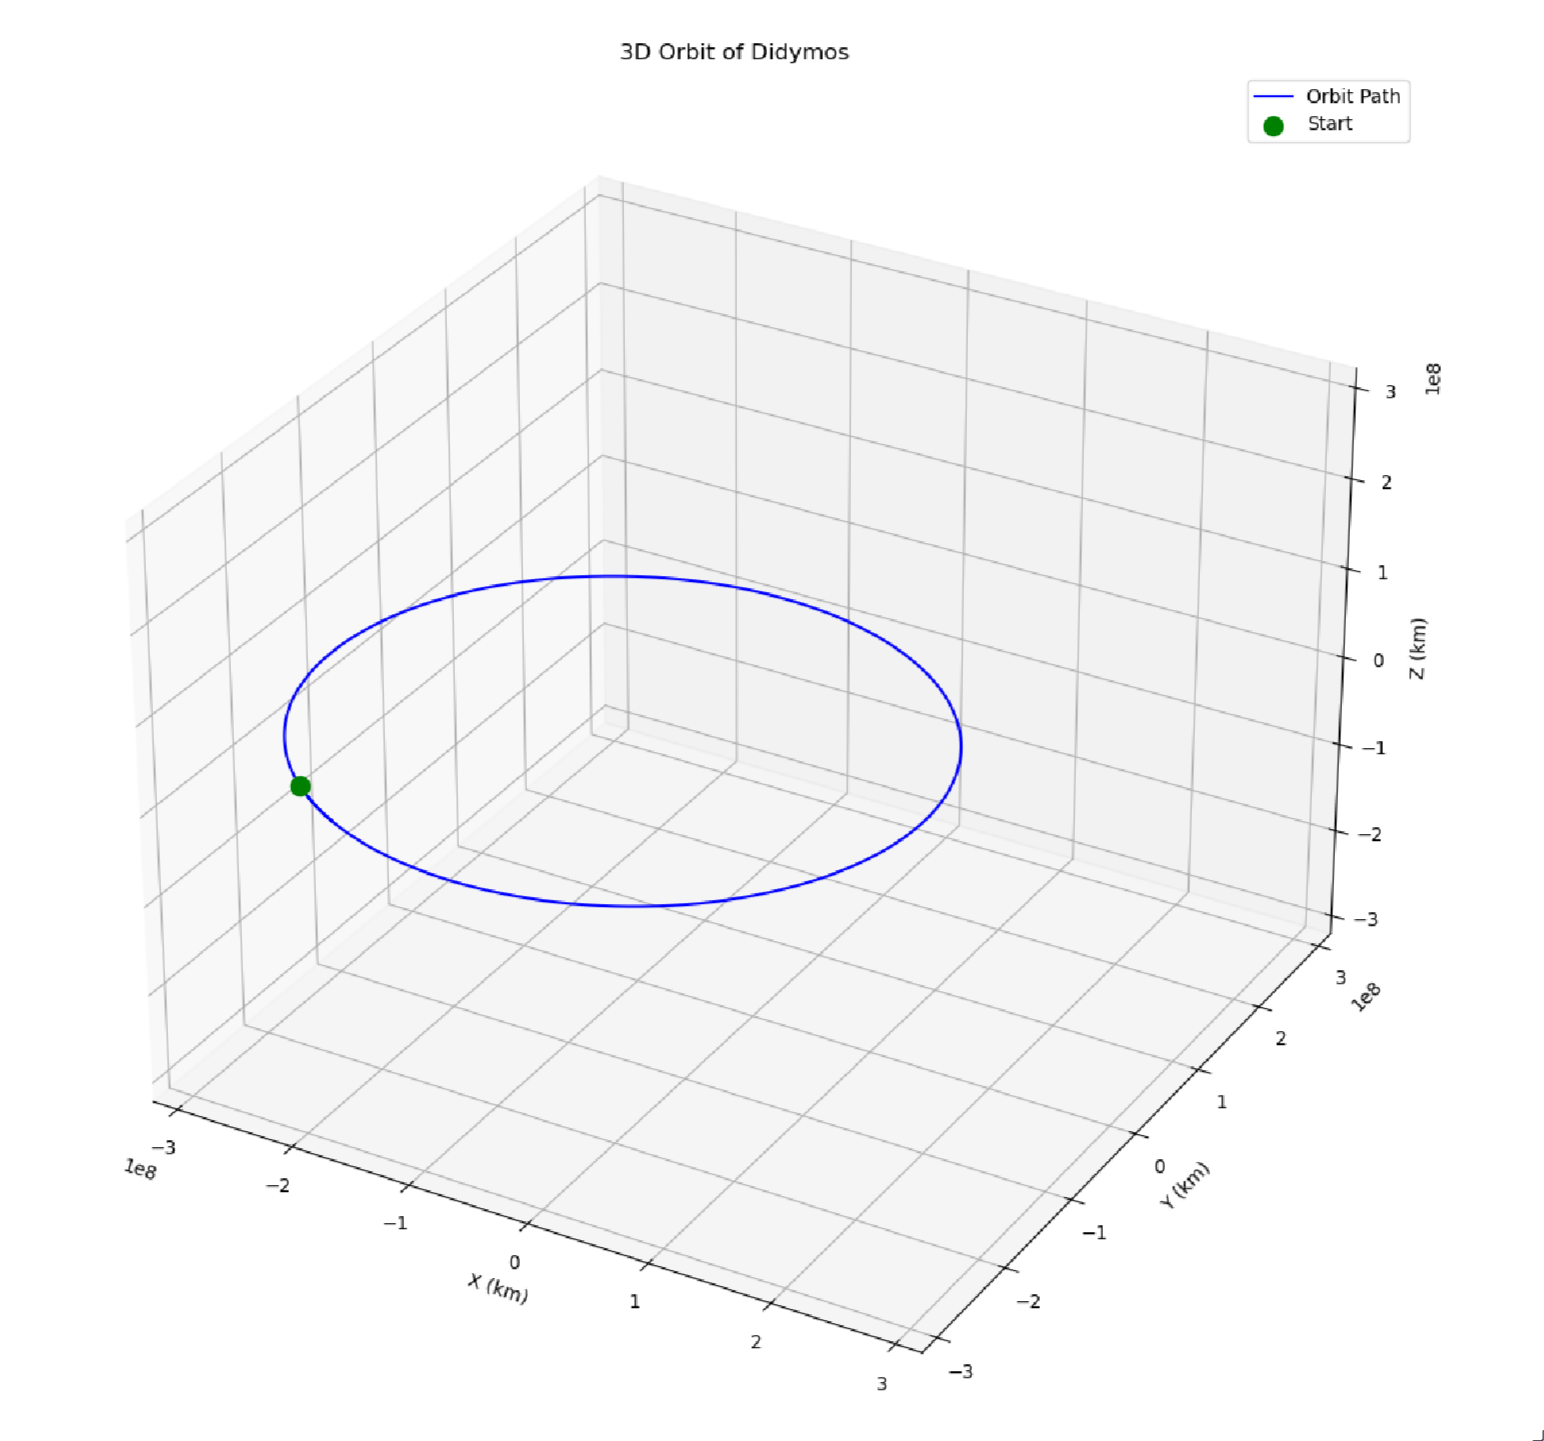
\includegraphics[width=0.45\textwidth]{./images/s02b.png}
		\end{center}
		\caption{Osculating orbital elements for orbit of Didymos}\label{fig:s02b}
	\end{figure}

	\hwkPart

	\begin{figure}[H]
		\begin{center}
			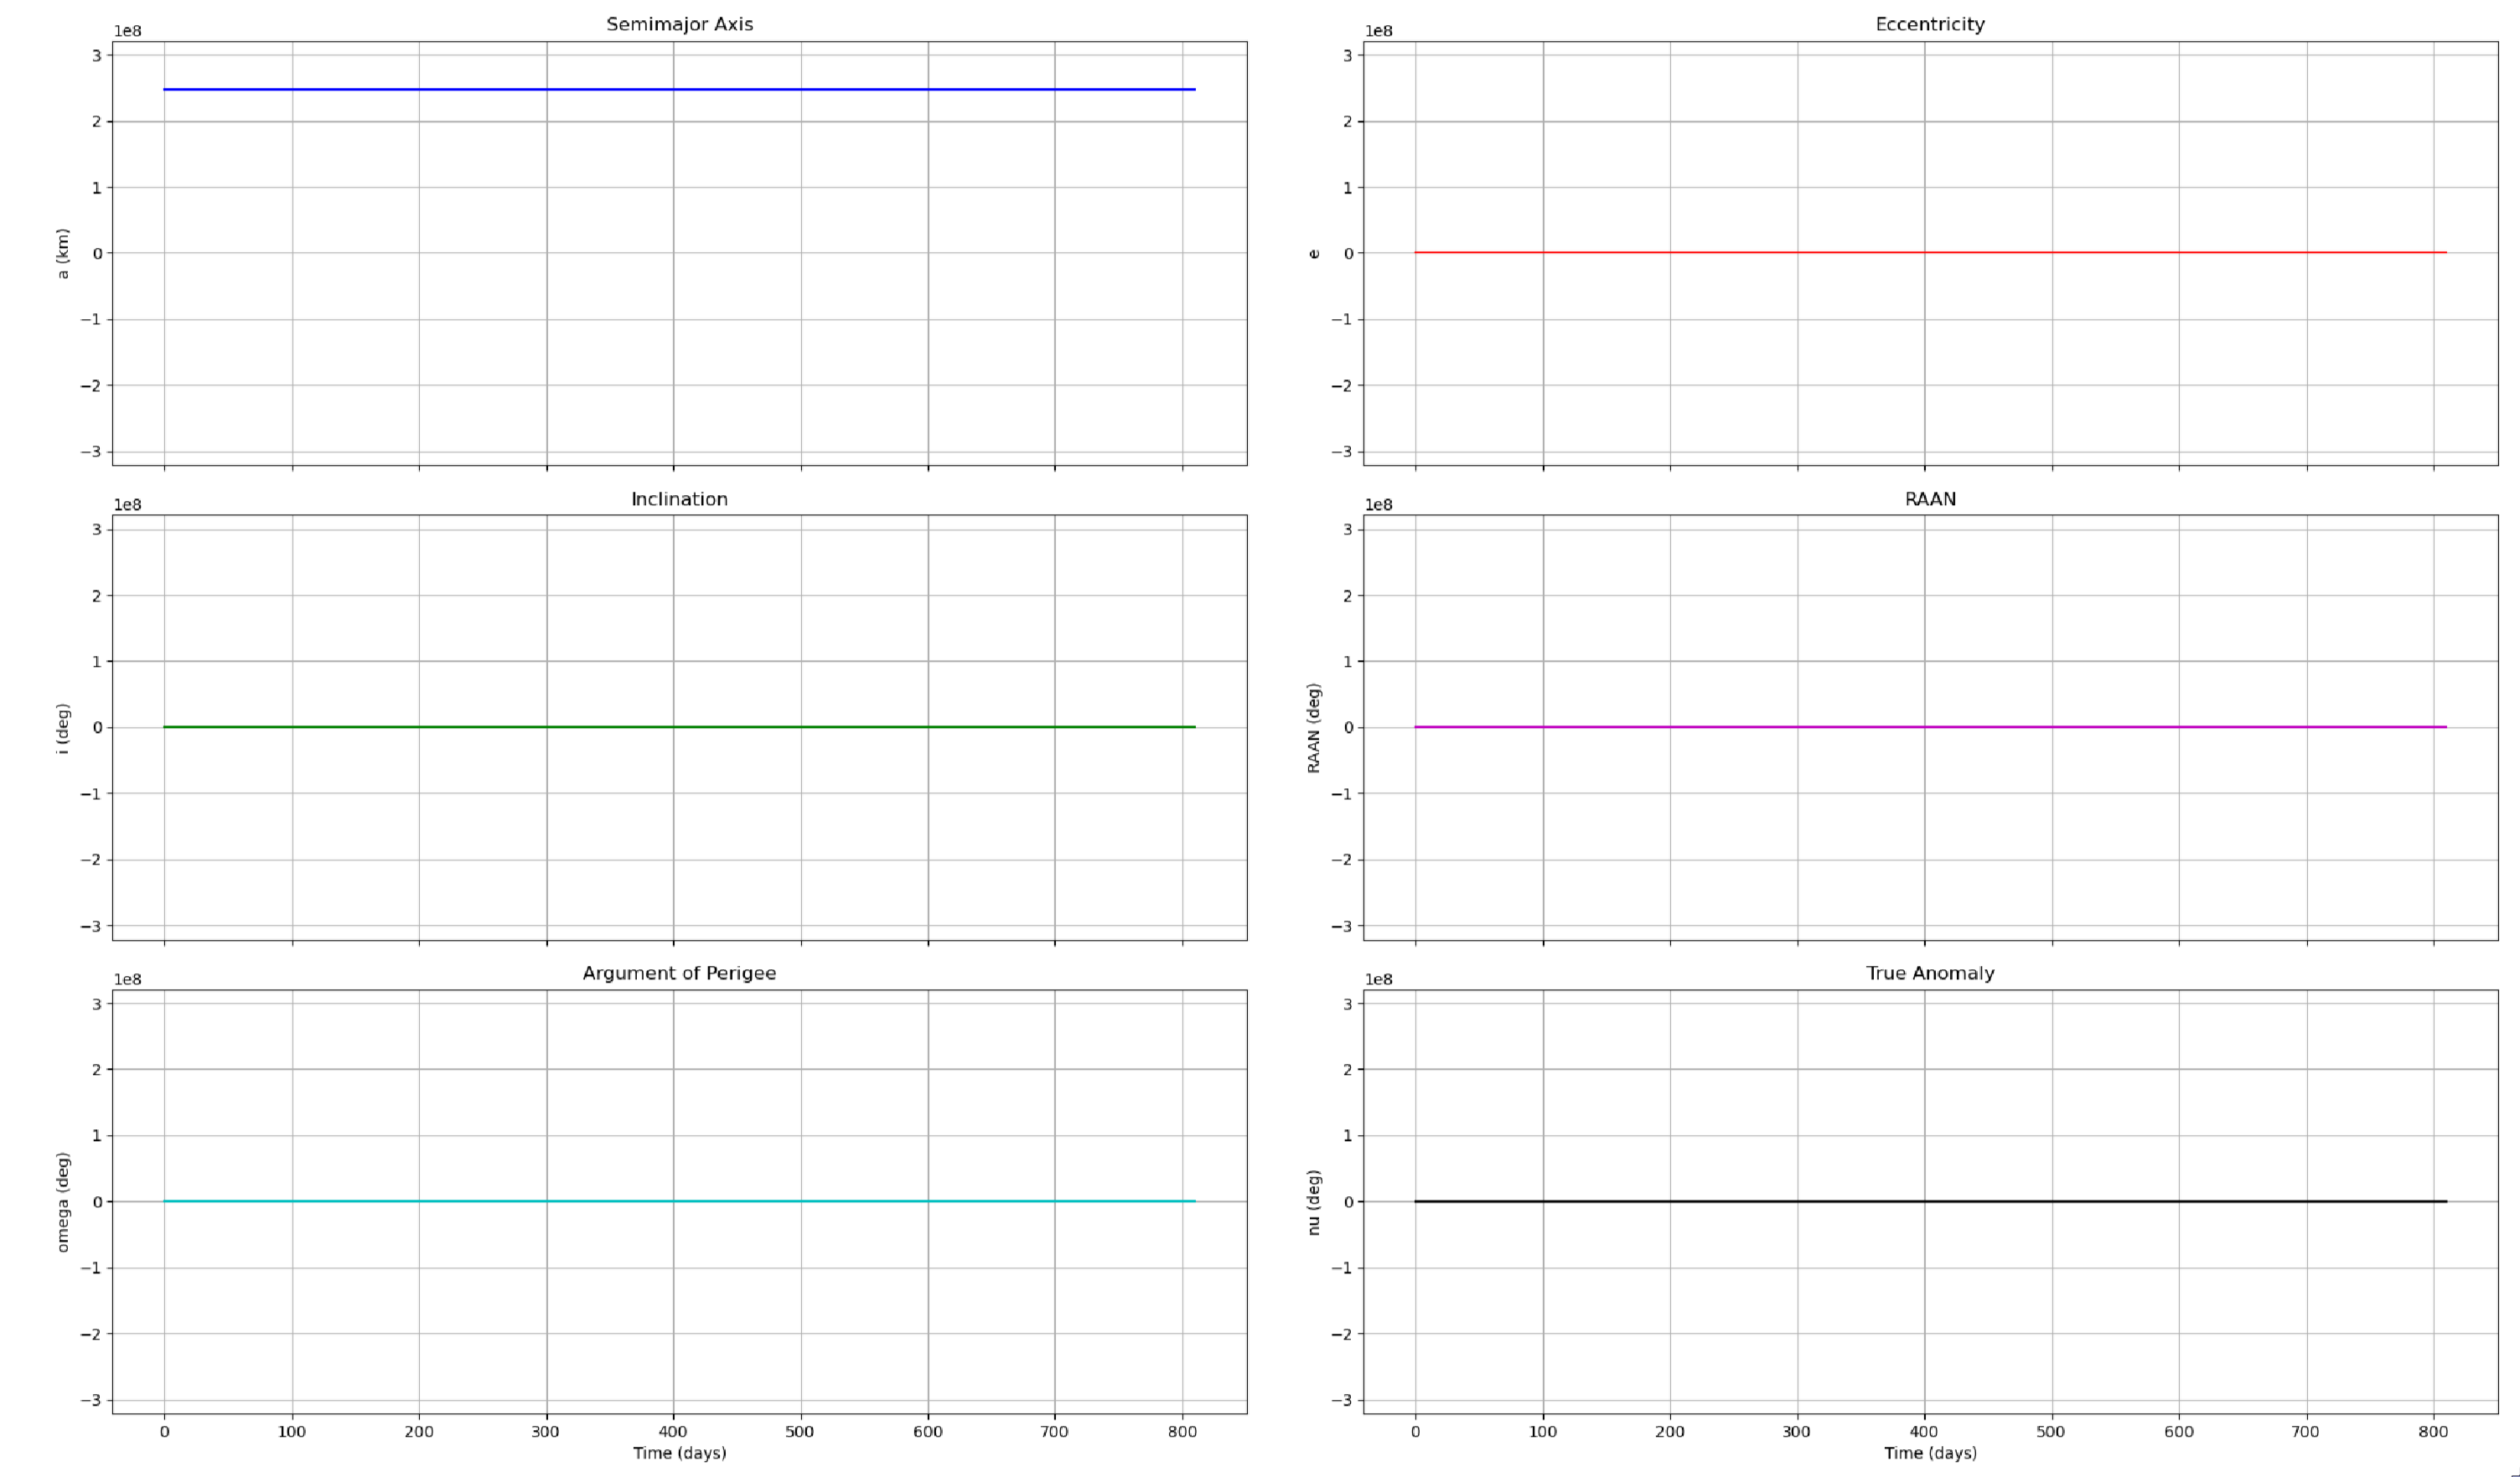
\includegraphics[width=0.85\textwidth]{./images/s02c.png}
		\end{center}
		\caption{Osculating orbital elements for orbit of Didymos}\label{fig:s02c}
	\end{figure}

	The 3D plot shows a complete elliptical path. This is consistent with Kepler’s first law: objects in a two‐body problem follow elliptical orbits around the central body. The starting point is clearly marked, and the overall shape confirms the stability of the orbit under the chosen initial conditions.

	In a perfect two-body system, the semimajor axis and eccentricity (which define the size and shape of the ellipse) remain constant. The inclination, RAAN, and argument of perigee, which determine the orbit’s orientation, should also remain constant (except for the continuous increase in true anomaly as the body moves along the orbit). The subplots show smooth variations—especially the true anomaly’s continuous growth—which confirm that the simulation captures the expected periodic and nearly constant behavior of the other elements. Slight numerical variations can be seen due to the integration method, but overall, the behavior is consistent with the theory.

\end{hwkProblem}
\begin{hwkProblem}{3}{}

	Given the following orbit: \( a=\qty{2e4}{\km}, e=0.4, i=\qty{100}{\degree}, \Omega=\qty{30}{\degree}, \omega=\qty{15}{\degree}, \nu=\qty{15}{\degree} \)
	\begin{enumerate}
		\item Write code to convert from orbital elements to Cartesian coordinates.
		\item Propogate the orbit (around Earth) for one period.
		\item State the period of the orbit.
		\item Plot the orbit in 3D (use equal-length axes).
		\item Plot the deviation of the energy as compared to the inital energy \( \left( E_i - E_0 \right) \).
		\item Plot the osculating orbital elements.
	\end{enumerate}

	\hwkSol

	\hwkPart

	See code in Listing \ref{lst:s03}

	\hwkPart

	See code in Listing \ref{lst:s03}

	\hwkPart

	Orbital period: \qty{7.82}{\hour}

	\hwkPart

	\begin{figure}[H]
		\begin{center}
			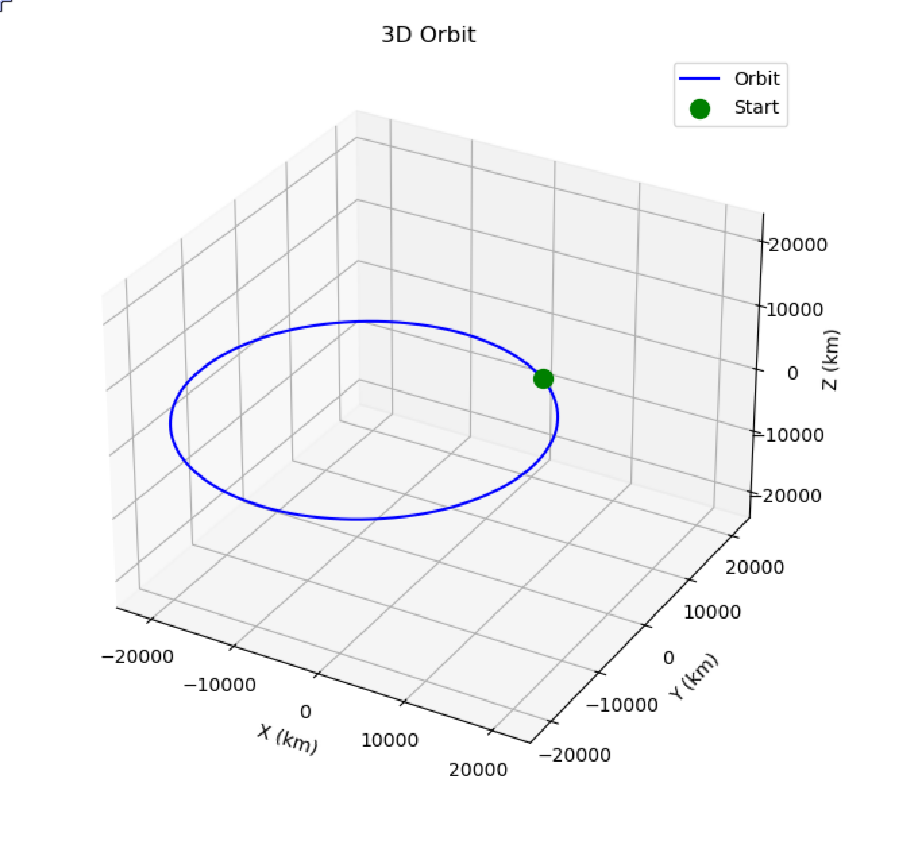
\includegraphics[width=0.65\textwidth]{./images/s03d.png}
		\end{center}
		\caption{3D Orbit about Earth}\label{fig:s03d}
	\end{figure}

	\hwkPart

	\begin{figure}[H]
		\begin{center}
			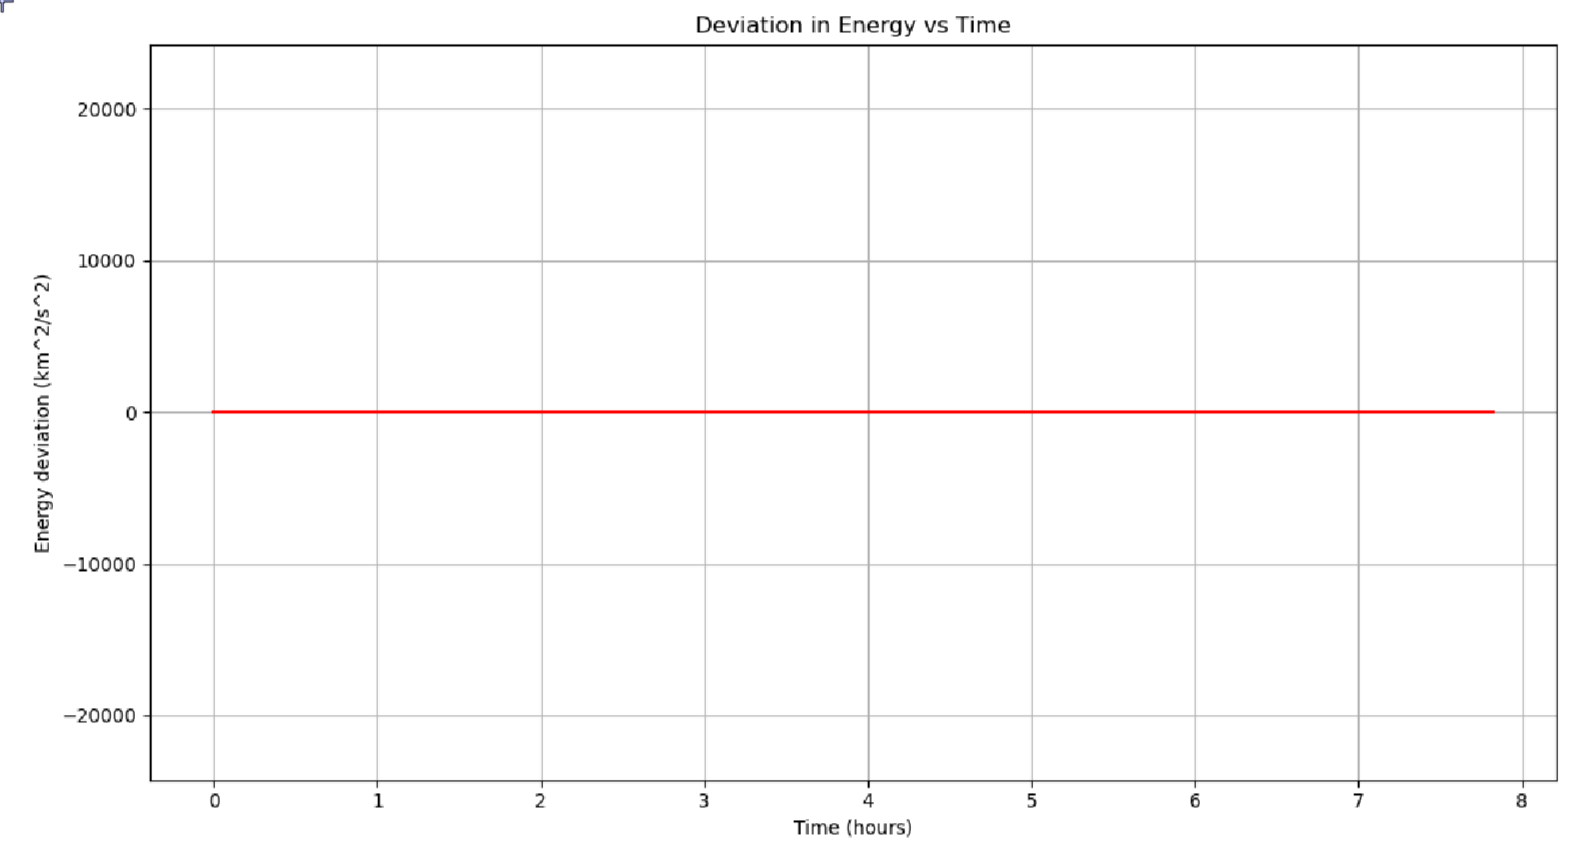
\includegraphics[width=0.65\textwidth]{./images/s03e.png}
		\end{center}
		\caption{Deviation of Energy w.r.t. Initial Energy \( \left( E_{i} - E_{0} \right)  \)}\label{fig:s03e}
	\end{figure}

	\hwkPart

	\begin{figure}[H]
		\begin{center}
			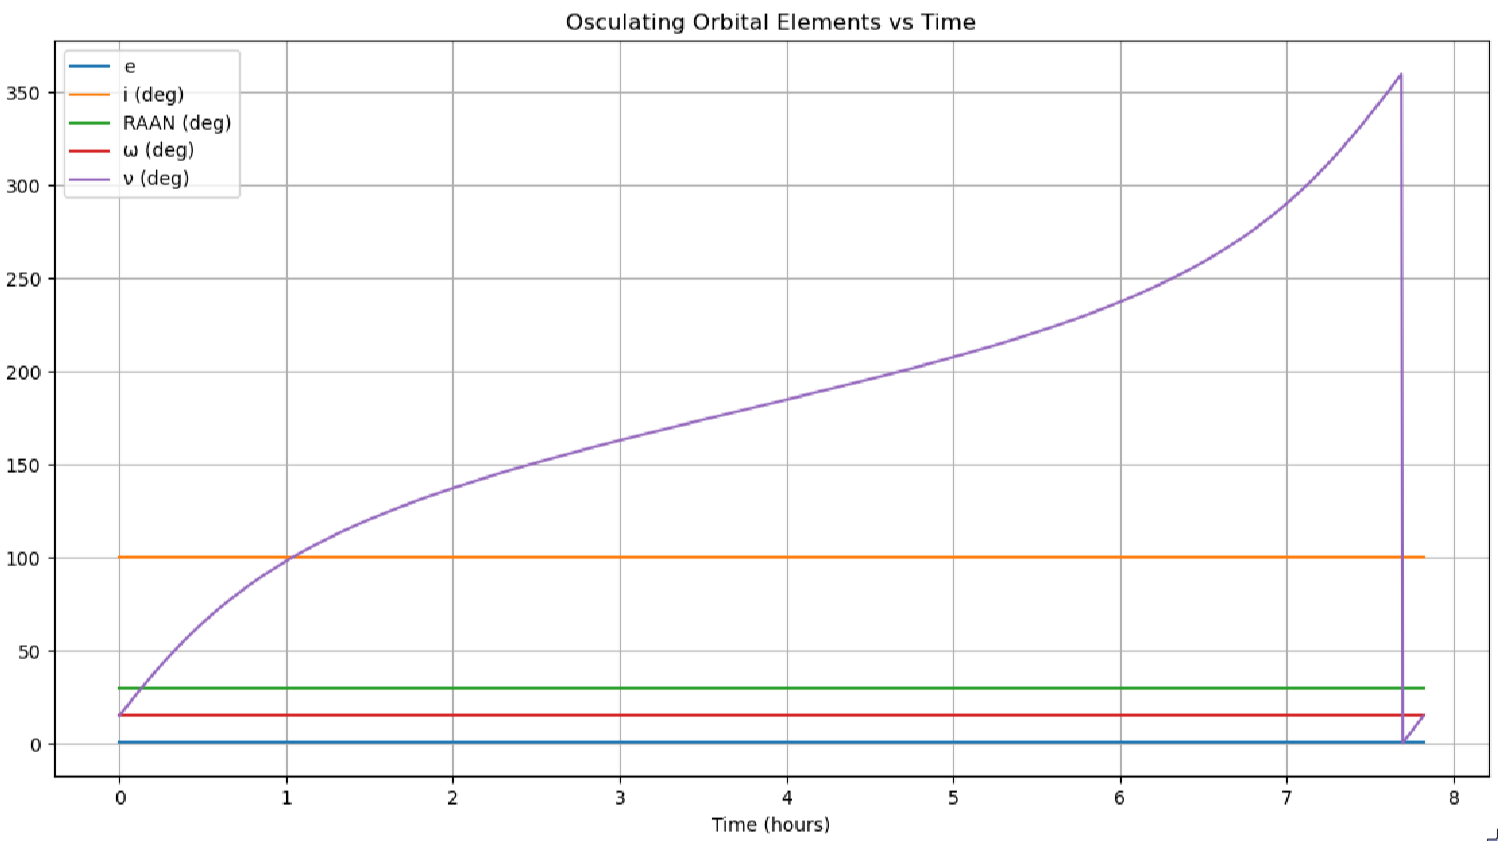
\includegraphics[width=0.65\textwidth]{./images/s03f.png}
		\end{center}
		\caption{Oscilating Orbital Elements}\label{fig:s03f}
	\end{figure}

	\vspace{\baselineskip / 2}
	\textbf{\large Code}
	\vspace{\baselineskip / 2}

	\lstinputlisting[language=python, caption={Python code for HW02 P03}, label={lst:s03}]{./code/s03.py}

\end{hwkProblem}
\begin{hwkProblem}{4}{}
	Sketch the following orbits in 2D and 3D. Assume that none of the spacecraft impact Earth.
	\begin{itemize}
		\item In the 2D orbit, label:
			\begin{itemize}
				\item periapsis
				\item angular momentum vector
				\item ascending node
				\item descending node
				\item spacecraft location
				\item portion of the orbit in the southern hemisphere
			\end{itemize}
		\item In the 3D orbit, label:
			\begin{itemize}
				\item angular momentum vector
				\item ascending node
				\item periapsis
			\end{itemize}
	\end{itemize}
	\begin{center}
		\begin{tabular}{cccccc}
			\hline
			Spacecraft ID & e & \(\mathrm{i} \left( \unit{\degree} \right) \) & \(\Omega \left( \unit{\degree} \right)\) & \(\omega \left( \unit{\degree} \right)\) & \(\nu \left( \unit{\degree} \right)\) \\
			\hline
			\hline
			A & 0.3 & 60 & 30 & 160 & 30 \\
			\hline
			B & 0.3 & 60 & 330 & 90 & 10 \\
			\hline
			C & 0.5 & 120 & 30 & 30 & 180 \\
			\hline
		\end{tabular}
	\end{center}

	\hwkSol

	\hwkPart

	\begin{figure}[H]
		\begin{center}
			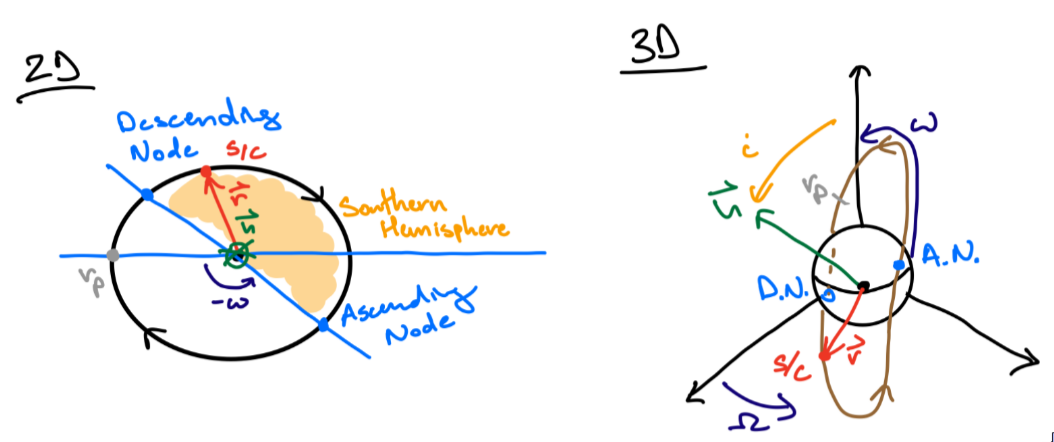
\includegraphics[width=0.65\textwidth]{./images/s04a.png}
		\end{center}
		\caption{Spacecraft A Orbit in 2D (left) and 3D (right)}\label{fig:s04a}
	\end{figure}

	\hwkPart

	\begin{figure}[H]
		\begin{center}
			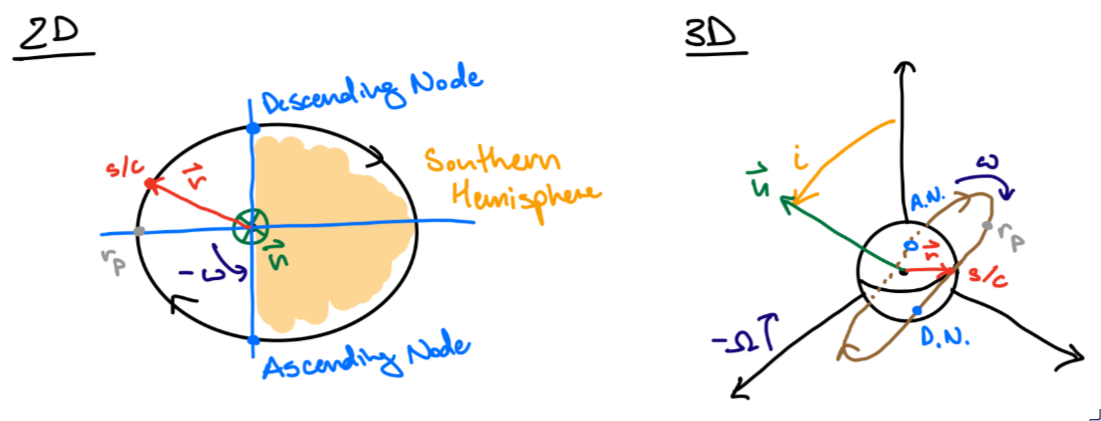
\includegraphics[width=0.65\textwidth]{./images/s04b.png}
		\end{center}
		\caption{Spacecraft B Orbit in 2D (left) and 3D (right)}\label{fig:s04b}
	\end{figure}

	\hwkPart

	\begin{figure}[H]
		\begin{center}
			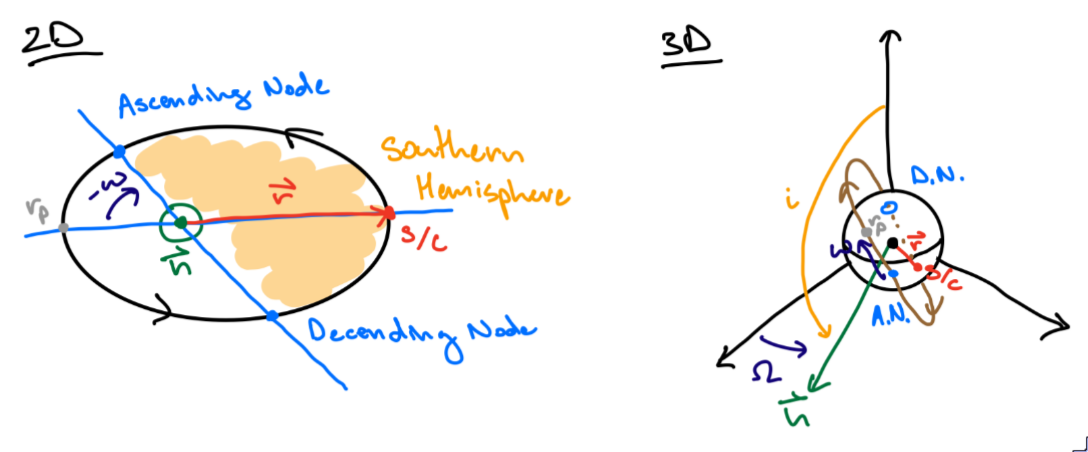
\includegraphics[width=0.65\textwidth]{./images/s04c.png}
		\end{center}
		\caption{Spacecraft C Orbit in 2D (left) and 3D (right)}\label{fig:s04c}
	\end{figure}

\end{hwkProblem}
\begin{hwkProblem}{5}{}

	Consider a spacecraft on a hyperbolic trajectory that will fly by Mars. The trajectory's semi-major axis is \qty{-11e3}{\km} and its eccentricity is \( 1.8 \). Calculate:
	\begin{enumerate}
		\item Turn angle
		\item Hyperbolic excess speed
		\item Miss distance
		\item Radius of periapsis of the flyby
	\end{enumerate}

	\hwkSol

	\hwkPart

	\begin{align*}
		a = \qty{-11e3}{\km} \\
		e = 1.8 \\
		\frac{1}{e} = \sin{\frac{\delta}{2}} \\
		\delta = 2 \sin^{-1}{\frac{1}{e}} = \qty{67.50}{\degree} \qed
	\end{align*}

	\hwkPart

	\begin{align*}
		\mu = \qty{4.282837e4}{\cubic\km\per\square\s} \\
		v_{\infty} = \sqrt{\frac{-\mu}{a}} = \qty{1.973}{\km\per\s} \qed
	\end{align*}

	\hwkPart

	\begin{align*}
		p = a \left( 1 - e^{2} \right) = \qty{24640}{\km} \\
		h = \sqrt{\mu p} = \qty{32485.86}{\square\km\per\s} \\
		h = v_{\infty} \Delta \\
		\Delta = \frac{h}{v_{\infty}} = \qty{16463}{\km} \qed
	\end{align*}

	\hwkPart

	\begin{align*}
		r_{p} = a \left( 1 - e \right) = \qty{8800}{\km} \qed
	\end{align*}

\end{hwkProblem}
\begin{hwkProblem}{6}{}

	Give the orbital element for an Earth-orbiting spacecraft crossing the \( \bm{\hat{y}} \) axis in a retrograde, equatorial, circular orbit at an altitude of \( \qty{1}{\DU} \). All angles should be given in degrees.
	\begin{enumerate}
		\item What is the semi-major axis (in DU)?
		\item Eccentricity?
		\item Inclination?
		\item Logitude of the ascending node?
		\item Argument of periapsis?
		\item True anomaly?
		\item True longitude at epoch?
	\end{enumerate}

	\hwkSol

	\hwkPart

	Circular orbit \( \therefore a = \qty{2}{\DU} \qed \)

	\hwkPart

	Circular orbit \( \therefore e = 0 \qed \)

	\hwkPart

	Retrograde orbit \( \therefore i = \qty{180}{\degree} \qed \)

	\hwkPart

	Equatorial orbit \( \therefore \Omega = 0 \qed \)

	\hwkPart

	Circular orbit \( \therefore \omega = 0 \qed \)

	\hwkPart

	Crossing the \( \bm{\hat{y}} \) axis \( \therefore \nu = \qty{270}{\degree} \qed \)

	\hwkPart

	Crossing the \( \bm{\hat{y}} \) axis \( \therefore L = \qty{270}{\degree} \qed \)

\end{hwkProblem}
\begin{hwkProblem}{7}{}

	Match the following orbits to the descriptions below:
	\begin{center}
		\begin{tabular}{cccccc}
			\hline
			Spacecraft ID & e & \(\mathrm{i} \left( \unit{\degree} \right) \) & \(\Omega \left( \unit{\degree} \right)\) & \(\omega \left( \unit{\degree} \right)\) & \(\nu \left( \unit{\degree} \right)\) \\
			\hline
			\hline
			A & 1 & 60 & 180 & 160 & 30 \\
			\hline
			B & 2 & 160 & 260 & 90 & 10 \\
			\hline
			C & 0.5 & 20 & 210 & 30 & 180 \\
			\hline
			D & 0.2 & 90 & 110 & 210 & 270 \\
			\hline
		\end{tabular}
	\end{center}
	\begin{enumerate}
		\item This is a retrograde orbit
		\item This spacecraft currently has a positive flight path angle
		\item This spacecraft is currently in the southern hemisphere
		\item This spacecraft is currently at apoapsis
		\item This orbit has a periapsis in the southern hemisphere
		\item This orbit has a line of nodes that is colinear with \( \bm\hat{{x}} \)
	\end{enumerate}

	\hwkSol

	\begin{enumerate}
		\item B
		\item A, B
		\item A, C
		\item C
		\item D
		\item A
	\end{enumerate}

\end{hwkProblem}
\begin{hwkProblem}{8}{}

	Given an elliptical orbit about the Earth with an eccentricity of \( 0.3 \) and a radius of periapsis of \qty{8000}{\km}, calculate the time of flight of the following:
	\begin{enumerate}
		\item From \( \nu = \qty{20}{\degree} \to \qty{30}{\degree} \)
		\item From \( \nu = \qty{300}{\degree} \to \qty{20}{\degree} \)
	\end{enumerate}

	\hwkSol

	\hwkPart

	\begin{align*}
		\nu = \qty{30}{\degree} \\
		\nu_{0} = \qty{20}{\degree} \\
		k = 0 \\
		\mu = \qty{3.986e5}{\cubic\km\per\square\s} \\
		E = \arccos{\left(\frac{e+\cos{\left(\nu\right)}}{1+e\cos{\left(\nu\right)}}\right)} = \qty{0.3883}{\radian} \\
		E_{0} = \arccos{\left(\frac{e+\cos{\left(\nu _{0}\right)}}{1+e\cos{\left(\nu_{0}\right)}}\right)} = \qty{0.2573}{\radian} \\
		r_{p} = a \left(1 - e\right) \implies a = \frac{r_{p}}{1-e} = \qty{11428.57}{\km} \\
		\Delta T = \sqrt{\frac{a^{3}}{\mu}} \left(2k\pi+\left(E-e\sin{\left(E\right)}\right) - \left(E_{0} - e \sin{\left(E_{0}\right)}\right)\right) = \qty{181.35}{\s} \qed
	\end{align*}

	\hwkPart

	\begin{align*}
		\nu = \qty{20}{\degree} \\
		\nu_{0} = \qty{300}{\degree} \\
		k = 1 \\
		E = \arccos{\left( \frac{e+\cos{\left(\nu\right)}}{1+e\cos{\left(\nu\right)}} \right)} = \qty{0.2573}{\radian} \\
		E_{0} = \arccos{\left(\frac{e+\cos{\left(\nu_{0}\right)}}{1+e\cos{\left(\nu_{0}\right)}}\right)} = \qty{-0.80147}{\radian} \implies E_{0} = 2\pi+\left(-0.80147\right) = \qty{5.4817}{\radian} \\
		\Delta T = \sqrt{\frac{a^{3}}{\mu}} \left(2k\pi+\left(E-e\sin{\left(E\right)}\right) - \left(E_{0} - e \sin{\left(E_{0}\right)}\right)\right) = \qty{1484.2}{\s} \qed
	\end{align*}

\end{hwkProblem}
\end{document}
